\documentclass{standalone}
\usepackage[utf8]{inputenc}
\usepackage{pgfplots}
\DeclareUnicodeCharacter{2212}{-}
\usepgfplotslibrary{groupplots,dateplot,polar}
\usetikzlibrary{patterns,shapes.arrows,arrows.meta}
\pgfplotsset{compat=newest}
\begin{document}
% This file was created with makintikz v1.0.1.
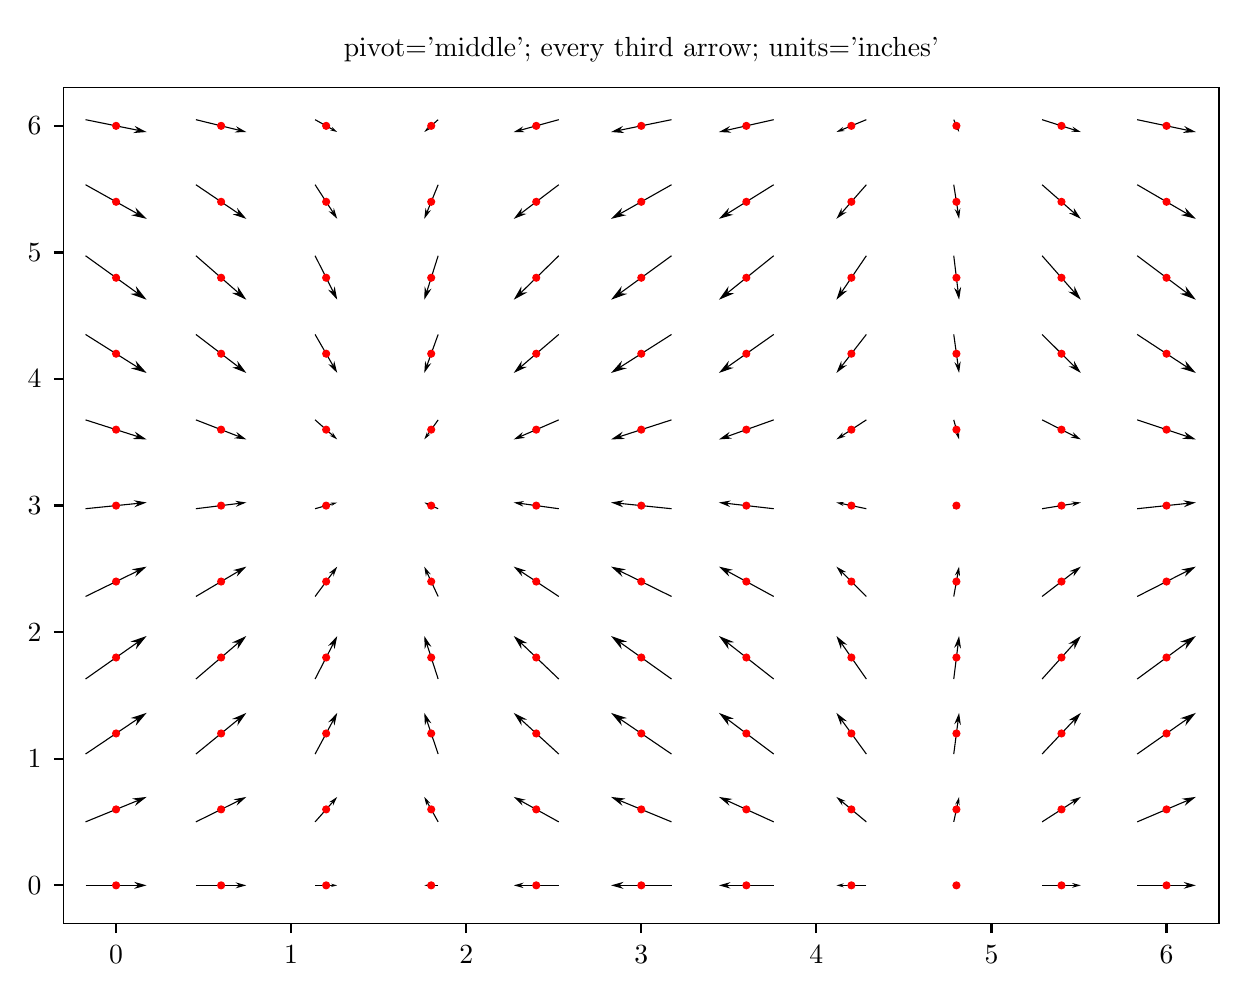
\begin{tikzpicture}

\definecolor{darkgray176}{RGB}{176,176,176}

\pgfkeys{/pgf/number format/std=-5:6, /pgf/number format/precision=5}

\begin{axis}[
height=4.8in,
minor xtick={},
minor ytick={},
scale ticks above exponent=5,
scale ticks below exponent=-4,
tick align=outside,
tick pos=left,
title={pivot='middle'; every third arrow; units='inches'},
width=6.4in,
x grid style={darkgray176},
xmin=-0.3, xmax=6.3,
xtick style={color=black, /pgfplots/major tick length=3.5pt, line width=0.8pt},
xtick={-1,0,1,2,3,4,5,6,7},
xticklabel shift=3.5pt,
xticklabel style={inner sep=0pt, yshift=0pt, anchor=north},
y grid style={darkgray176},
ymin=-0.3, ymax=6.3,
ytick style={color=black, /pgfplots/major tick length=3.5pt, line width=0.8pt},
ytick={-1,0,1,2,3,4,5,6,7},
yticklabel shift=3.5pt,
yticklabel style={inner sep=0pt, xshift=0pt}
]
\addplot [
point meta={sqrt((\thisrow{u})^2 + (\thisrow{v})^2)},
quiver={
u=\thisrow{u},v=\thisrow{v},
scale arrows=0.34891067819001353,
every arrow/.append style={
   -{Stealth[
      scale length={0.25 + 1.0 * \pgfplotspointmetatransformed / 1000},
      scale width={0.15 + 0.8 * \pgfplotspointmetatransformed / 1000}
   ]}
}},
black
]
table [x expr={\thisrow{x} - 0.5 * 0.34891067819001353 * \thisrow{u}},y expr={\thisrow{y} - 0.5 * 0.34891067819001353 * \thisrow{v}}] {%
x y u v
0 0 1 0
0.6 0 0.825335614909678 0
1.2 0 0.362357754476673 0
1.8 0 -0.227202094693087 0
2.4 0 -0.737393715541246 0
3 0 -0.989992496600445 0
3.6 0 -0.896758416334147 0
4.2 0 -0.490260821340699 0
4.8 0 0.0874989834394473 0
5.4 0 0.634692875942635 0
6 0 0.960170286650366 0
0 0.6 1 0.564642473395035
0.6 0.6 0.825335614909678 0.564642473395035
1.2 0.6 0.362357754476673 0.564642473395035
1.8 0.6 -0.227202094693087 0.564642473395035
2.4 0.6 -0.737393715541246 0.564642473395035
3 0.6 -0.989992496600445 0.564642473395035
3.6 0.6 -0.896758416334147 0.564642473395035
4.2 0.6 -0.490260821340699 0.564642473395035
4.8 0.6 0.0874989834394473 0.564642473395035
5.4 0.6 0.634692875942635 0.564642473395035
6 0.6 0.960170286650366 0.564642473395035
0 1.2 1 0.932039085967226
0.6 1.2 0.825335614909678 0.932039085967226
1.2 1.2 0.362357754476673 0.932039085967226
1.8 1.2 -0.227202094693087 0.932039085967226
2.4 1.2 -0.737393715541246 0.932039085967226
3 1.2 -0.989992496600445 0.932039085967226
3.6 1.2 -0.896758416334147 0.932039085967226
4.2 1.2 -0.490260821340699 0.932039085967226
4.8 1.2 0.0874989834394473 0.932039085967226
5.4 1.2 0.634692875942635 0.932039085967226
6 1.2 0.960170286650366 0.932039085967226
0 1.8 1 0.973847630878195
0.6 1.8 0.825335614909678 0.973847630878195
1.2 1.8 0.362357754476673 0.973847630878195
1.8 1.8 -0.227202094693087 0.973847630878195
2.4 1.8 -0.737393715541246 0.973847630878195
3 1.8 -0.989992496600445 0.973847630878195
3.6 1.8 -0.896758416334147 0.973847630878195
4.2 1.8 -0.490260821340699 0.973847630878195
4.8 1.8 0.0874989834394473 0.973847630878195
5.4 1.8 0.634692875942635 0.973847630878195
6 1.8 0.960170286650366 0.973847630878195
0 2.4 1 0.675463180551151
0.6 2.4 0.825335614909678 0.675463180551151
1.2 2.4 0.362357754476673 0.675463180551151
1.8 2.4 -0.227202094693087 0.675463180551151
2.4 2.4 -0.737393715541246 0.675463180551151
3 2.4 -0.989992496600445 0.675463180551151
3.6 2.4 -0.896758416334147 0.675463180551151
4.2 2.4 -0.490260821340699 0.675463180551151
4.8 2.4 0.0874989834394473 0.675463180551151
5.4 2.4 0.634692875942635 0.675463180551151
6 2.4 0.960170286650366 0.675463180551151
0 3 1 0.141120008059867
0.6 3 0.825335614909678 0.141120008059867
1.2 3 0.362357754476673 0.141120008059867
1.8 3 -0.227202094693087 0.141120008059867
2.4 3 -0.737393715541246 0.141120008059867
3 3 -0.989992496600445 0.141120008059867
3.6 3 -0.896758416334147 0.141120008059867
4.2 3 -0.490260821340699 0.141120008059867
4.8 3 0.0874989834394473 0.141120008059867
5.4 3 0.634692875942635 0.141120008059867
6 3 0.960170286650366 0.141120008059867
0 3.6 1 -0.442520443294852
0.6 3.6 0.825335614909678 -0.442520443294852
1.2 3.6 0.362357754476673 -0.442520443294852
1.8 3.6 -0.227202094693087 -0.442520443294852
2.4 3.6 -0.737393715541246 -0.442520443294852
3 3.6 -0.989992496600445 -0.442520443294852
3.6 3.6 -0.896758416334147 -0.442520443294852
4.2 3.6 -0.490260821340699 -0.442520443294852
4.8 3.6 0.0874989834394473 -0.442520443294852
5.4 3.6 0.634692875942635 -0.442520443294852
6 3.6 0.960170286650366 -0.442520443294852
0 4.2 1 -0.871575772413588
0.6 4.2 0.825335614909678 -0.871575772413588
1.2 4.2 0.362357754476673 -0.871575772413588
1.8 4.2 -0.227202094693087 -0.871575772413588
2.4 4.2 -0.737393715541246 -0.871575772413588
3 4.2 -0.989992496600445 -0.871575772413588
3.6 4.2 -0.896758416334147 -0.871575772413588
4.2 4.2 -0.490260821340699 -0.871575772413588
4.8 4.2 0.0874989834394473 -0.871575772413588
5.4 4.2 0.634692875942635 -0.871575772413588
6 4.2 0.960170286650366 -0.871575772413588
0 4.8 1 -0.996164608835841
0.6 4.8 0.825335614909678 -0.996164608835841
1.2 4.8 0.362357754476673 -0.996164608835841
1.8 4.8 -0.227202094693087 -0.996164608835841
2.4 4.8 -0.737393715541246 -0.996164608835841
3 4.8 -0.989992496600445 -0.996164608835841
3.6 4.8 -0.896758416334147 -0.996164608835841
4.2 4.8 -0.490260821340699 -0.996164608835841
4.8 4.8 0.0874989834394473 -0.996164608835841
5.4 4.8 0.634692875942635 -0.996164608835841
6 4.8 0.960170286650366 -0.996164608835841
0 5.4 1 -0.772764487555987
0.6 5.4 0.825335614909678 -0.772764487555987
1.2 5.4 0.362357754476673 -0.772764487555987
1.8 5.4 -0.227202094693087 -0.772764487555987
2.4 5.4 -0.737393715541246 -0.772764487555987
3 5.4 -0.989992496600445 -0.772764487555987
3.6 5.4 -0.896758416334147 -0.772764487555987
4.2 5.4 -0.490260821340699 -0.772764487555987
4.8 5.4 0.0874989834394473 -0.772764487555987
5.4 5.4 0.634692875942635 -0.772764487555987
6 5.4 0.960170286650366 -0.772764487555987
0 6 1 -0.279415498198926
0.6 6 0.825335614909678 -0.279415498198926
1.2 6 0.362357754476673 -0.279415498198926
1.8 6 -0.227202094693087 -0.279415498198926
2.4 6 -0.737393715541246 -0.279415498198926
3 6 -0.989992496600445 -0.279415498198926
3.6 6 -0.896758416334147 -0.279415498198926
4.2 6 -0.490260821340699 -0.279415498198926
4.8 6 0.0874989834394473 -0.279415498198926
5.4 6 0.634692875942635 -0.279415498198926
6 6 0.960170286650366 -0.279415498198926
};
\addplot [draw=red, fill=red, mark size=1.26156626101008pt, mark=*, only marks]
table{%
x  y
0 0
0.6 0
1.2 0
1.8 0
2.4 0
3 0
3.6 0
4.2 0
4.8 0
5.4 0
6 0
0 0.6
0.6 0.6
1.2 0.6
1.8 0.6
2.4 0.6
3 0.6
3.6 0.6
4.2 0.6
4.8 0.6
5.4 0.6
6 0.6
0 1.2
0.6 1.2
1.2 1.2
1.8 1.2
2.4 1.2
3 1.2
3.6 1.2
4.2 1.2
4.8 1.2
5.4 1.2
6 1.2
0 1.8
0.6 1.8
1.2 1.8
1.8 1.8
2.4 1.8
3 1.8
3.6 1.8
4.2 1.8
4.8 1.8
5.4 1.8
6 1.8
0 2.4
0.6 2.4
1.2 2.4
1.8 2.4
2.4 2.4
3 2.4
3.6 2.4
4.2 2.4
4.8 2.4
5.4 2.4
6 2.4
0 3
0.6 3
1.2 3
1.8 3
2.4 3
3 3
3.6 3
4.2 3
4.8 3
5.4 3
6 3
0 3.6
0.6 3.6
1.2 3.6
1.8 3.6
2.4 3.6
3 3.6
3.6 3.6
4.2 3.6
4.8 3.6
5.4 3.6
6 3.6
0 4.2
0.6 4.2
1.2 4.2
1.8 4.2
2.4 4.2
3 4.2
3.6 4.2
4.2 4.2
4.8 4.2
5.4 4.2
6 4.2
0 4.8
0.6 4.8
1.2 4.8
1.8 4.8
2.4 4.8
3 4.8
3.6 4.8
4.2 4.8
4.8 4.8
5.4 4.8
6 4.8
0 5.4
0.6 5.4
1.2 5.4
1.8 5.4
2.4 5.4
3 5.4
3.6 5.4
4.2 5.4
4.8 5.4
5.4 5.4
6 5.4
0 6
0.6 6
1.2 6
1.8 6
2.4 6
3 6
3.6 6
4.2 6
4.8 6
5.4 6
6 6
};
\end{axis}

\end{tikzpicture}

\end{document}